\PilotPage{22}

A rendition of the vertical vibration motion is depicted in Figure~3.

\setcounter{figure}{2}
\begin{figure}[!ht]
  \centering
  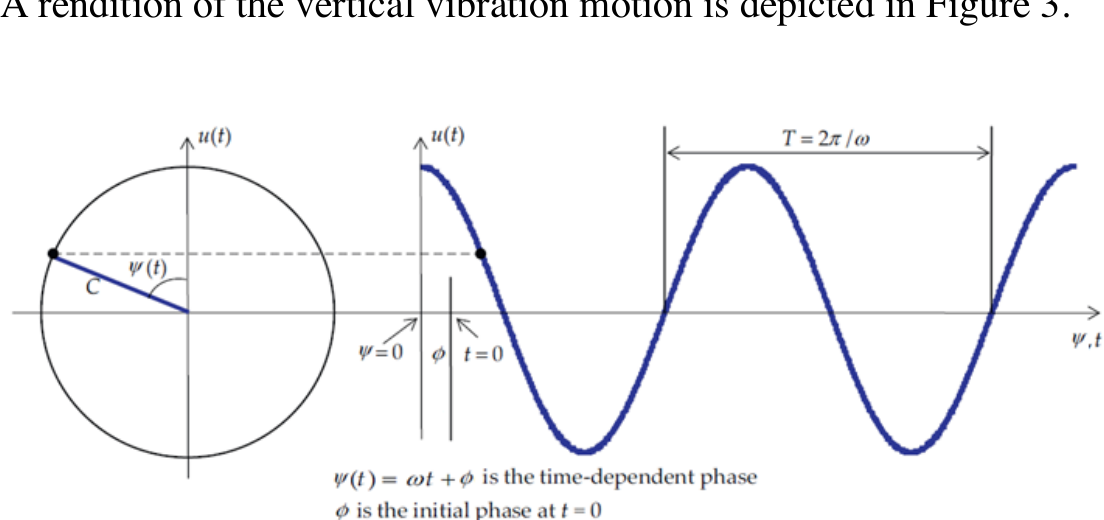
\includegraphics[
    trim=0 0 0 24bp,
    clip,
    max width=0.93\linewidth,
    max height=1.72in,
  ]{figures/p022-phase-motion.png}
  \caption{Schematic representation of an oscillatory motion of amplitude $C$, angular frequency $\omega$, and initial phase $\phi$}
\end{figure}

Note that the above analysis proved that the vibration equation is not modified if static gravity is also included in the analysis. This means that the vibration motion is not affected by the presence of a static force field such as gravity. The analysis can be easily extended to a static force field that is not parallel with the vibration motion, but it has an arbitrary orientation.
